\documentclass[dvipdfmx]{miyalab}

\usepackage{graphicx}
\usepackage{amssymb} % 記号

%\renewcommand{\baselinestretch}{1.0} % 行送りを倍率で設定
\setlength{\baselineskip}{9pt}       % 行送りを値で設定

% 表関連
\usepackage{colortbl,array,xcolor}
\usepackage{tabularx}
\newcolumntype{C}{>{\centering}X}
\renewcommand{\tabularxcolumn}[1]{m{#1}}
\usepackage{booktabs}

% 箇条書き
\usepackage{enumitem}

% レイアウトの確認
%\usepackage{layout}

\title{東京学芸大学 計算機科学研究室 (宮寺研究室) \LaTeX クラスファイル}
\etitle{Development of miyalab.cls}

\affiliation{宮寺研究室}
\studentid{R16-9003}
\author{佐藤 克己}
%\date{2017/7/25}

\begin{document}

\maketitle

\section{章のタイトル}
\subsection{節のタイトル}
\subsubsection{項のタイトル}

\section{箇条書き}

\begin{enumerate}[labelindent=1\parindent,leftmargin=*,label=第\arabic{enumi}位.,ref=\arabic{enumi}]
		\item つぶ貝\label{enum:item1}
		\item 赤貝\label{enum:item2}
		\item ミル貝\label{enum:item3}
\end{enumerate}

\ref{enum:item1} は...

\begin{enumerate}[labelindent=2\parindent,leftmargin=*,label=第\arabic{enumi}位.,ref=お寿司 その\arabic{enumi}]
		\item マグロ\label{enum:item4}
		\item カツオ\label{enum:item5}
		\item サーモン\label{enum:item6}
\end{enumerate}

\ref{enum:item4} は...

\section{引用}

\cite{miyalab-cls}

\cite{latex2e}

\section{図}

\begin{figure}[htbp]
\centering
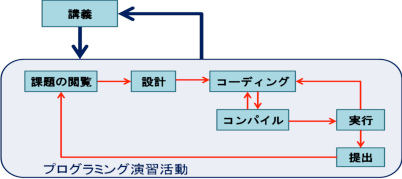
\includegraphics[width=\linewidth]{image/sample.pdf}
	\caption{サンプル画像 (PDF)}
	\label{fig:sample-pdf}
\end{figure}

\begin{figure}[htbp]
\centering
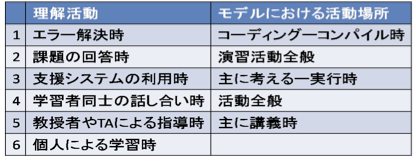
\includegraphics[width=\linewidth]{image/sample.png}
	\caption{サンプル画像 (PNG)}
	\label{fig:sample-png}
\end{figure}

画像の参照は, 図 \ref{fig:sample-pdf}, 図 \ref{fig:sample-png} のように行う。

\section{表}

表の例を表 \ref{tab:table-sample-booktabs}, \ref{tab:table-sample-rowcolor} に示す.

\begin{table}[htb]
	\caption{表の例}
	\label{tab:table-sample-booktabs}
	\begin{tabularx}{\linewidth}{CCC}
		\toprule
		\textbf{ヘッダ1} & \textbf{ヘッダ2} & \textbf{ヘッダ3}  \tabularnewline \midrule
		データ1          & データ1-1 \\
		                   データ1-2        & \checkmark        \tabularnewline \midrule
		データ2          & データ2-1 \\
		                   データ2-2        &                   \tabularnewline \midrule
		データ3          & データ3-1 \\
		                   データ3-2 \\
						   データ3-3        &                   \tabularnewline \midrule
		データ4          & データ4-1        &  \checkmark       \tabularnewline \midrule
		データ5          & データ5-1 \\ 
		                   データ5-2        &  \checkmark       \tabularnewline \bottomrule
	\end{tabularx}
\end{table}

\begin{table}[htb]
	\caption{表の例}
	\label{tab:table-sample-rowcolor}
	\begin{tabularx}{\linewidth}{|C|C|C|}
		\hline
		\rowcolor[gray]{0.8}
		\textbf{ヘッダ1} & \textbf{ヘッダ2} & \textbf{ヘッダ3}  \tabularnewline \hline
		データ1          & データ1-1 \\
		                   データ1-2        & \checkmark        \tabularnewline \hline
		データ2          & データ2-1 \\
		                   データ2-2        &                   \tabularnewline \hline
		データ3          & データ3-1 \\
		                   データ3-2 \\
						   データ3-3        &                   \tabularnewline \hline
		データ4          & データ4-1        &  \checkmark       \tabularnewline \hline
		データ5          & データ5-1 \\ 
		                   データ5-2        &  \checkmark       \tabularnewline \hline
	\end{tabularx}
\end{table}


\section{コメントアウト}

\begin{comment}
	この部分はコメントアウトされる
\end{comment}

\bibliographystyle{sieicej}

\bibliography{sample-bib}

\end{document}  
